\section{Introduction}
\label{sec:intro}
In Hypersonic flow in general, the mach number that is present is very high and the vehicles encounter variety of shock-shock interactions, shock wave boundary layer interactions, on a variety of configurations, On certain configuration that is on high aft and wedge angles, the frequency of the flows and presenting high amplitude and high viscous interactions, Many effects of high temperature features, Fatigue loading, uneven ablation of the walls on the re-entry vehicles including many shock shock interactions and shocks that are self sustaining which are fundamental for vehicle performance and efficiency.

Large number of experiments have been conducted on fins, hemispherical blunt body, aerospikes, compression ramps and over expanded nozzles are present and have been worked on for many years. Their main features was in the formation of separation bubble area variation and the entropy layer effects.[1]

\begin{figure}[ht]
\centering
  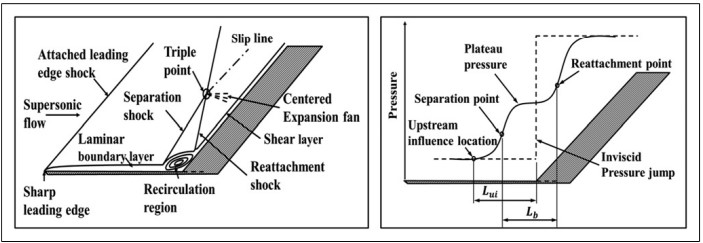
\includegraphics[width=0.8\linewidth]{images/photo.jpg}
  \caption{ Schematic diagram of ramp induced shock wave boundary layer interactions[2].}
  \label{fig:Schematic}
\end{figure}

In figure \ref{fig:Schematic}, the schematic diagram of shock wave boundary layer interaction on sharp leading edge ramp can be observed. If observed near the wall flow field, there is a compression corner and obliques hock interaction that can be observed, now this phenomenon is formed due to constant change of flows such as separation shock, there is an oblique shock formation in the tip of the cone or on the ramp that is present and if the ramp angle has a high angle but a short physical boundary then the oblique shock that is generated from the front cone plays an important role in the shock wave boundary layer interaction, Then after a few seconds into the run the oblique shock that is produced tend to hit the boundary layer of the aft wedge, there is a subsonic region created in the wedge centre of the double cone, Due to all the interactions happening the front and aft cone regions, the separation region or the subsonic region length changes and due to this a bow shock wave is formed in the front of the aft cone and this oblique shock and the bow shock interacts with each other and forms a triple point and due to this interaction a shear layer is formed in the aft cone and therefore an expansion fan is generated after the aft cone and there is an increase in the mach number. 